\section{時間分解能の式の評価}
\subsection{式の評価}

新たに、検出器由来のジッターの要素を加えた時間分解の式\ref{eq_TimingResolution}を定義した。
この式には、新たに信号由来のジッター$\sigma_m$と、時間分解能に影響を与える未知の要素$\sigma_x$を加えた。
この式で、LGAD検出器の時間分解能を表すことができるのか、それとも未知の要素$\sigma_x$が電圧に対してどのような振る舞いをするのかを
測定結果を用いて評価した。

\begin{equation}
    {\sigma_t}^2 = {\sigma_{tw}}^2 + {\sigma_j}^2 + {\sigma_L}^2+{\sigma_m}^2+{\sigma_x}^2
    \label{eq_TimingResolution}
\end{equation}

\subsection{未知の時間分解能の要素}
以下の図\ref{fg:unknownjittervsBias}に未知の時間分解能の要素$\sigma_x$の電圧依存性を示す。
PINは、
APDは、

\begin{figure}[h]
    \centering
    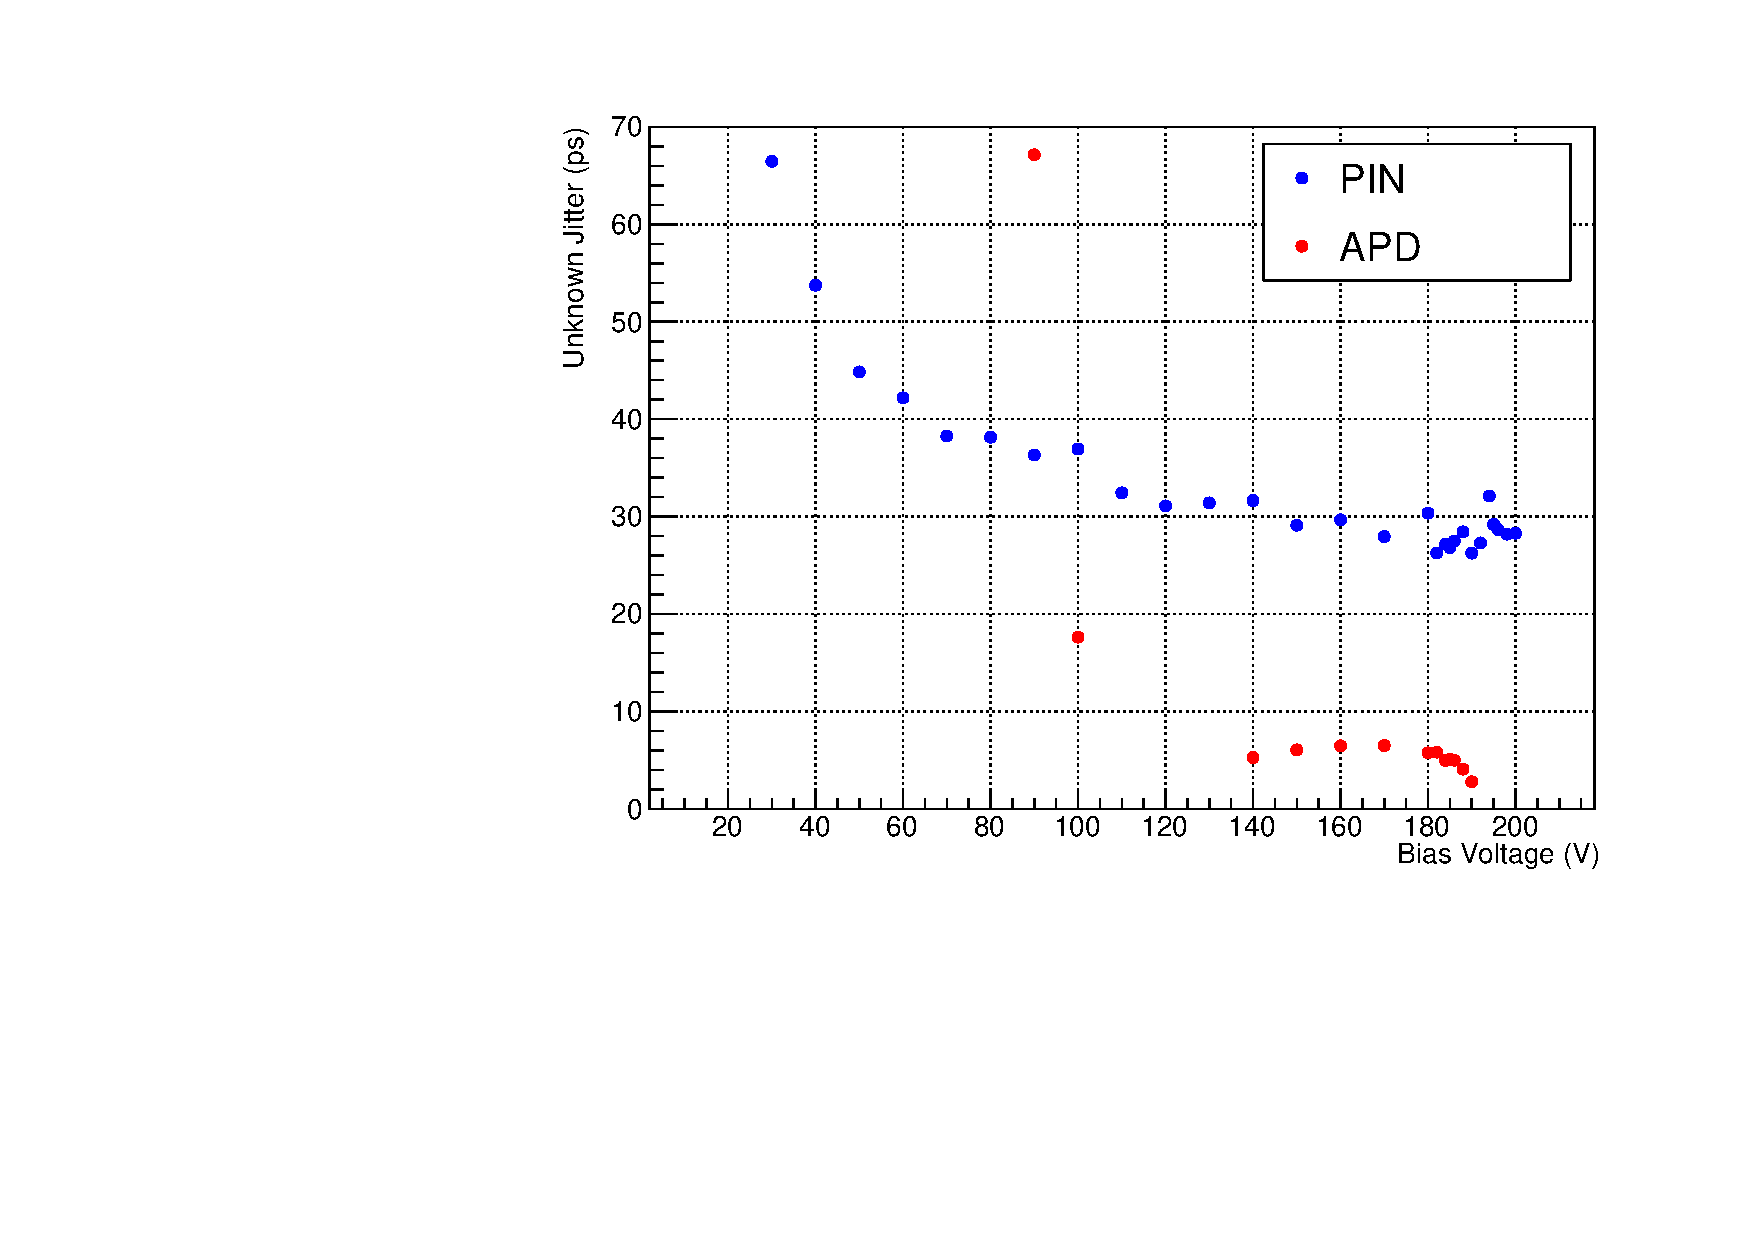
\includegraphics[width=8cm]{fig/graph/Unknownjitter_pad1ch_ver2_temp_126_20231220.pdf}
    \caption{未知の時間分解能の要素$\sigma_x$の電圧依存性}
    \label{fg:unknownjittervsBias}
\end{figure}


